\documentclass[border=2mm]{standalone}
\usepackage{tikz}
\usetikzlibrary{positioning}
\begin{document}
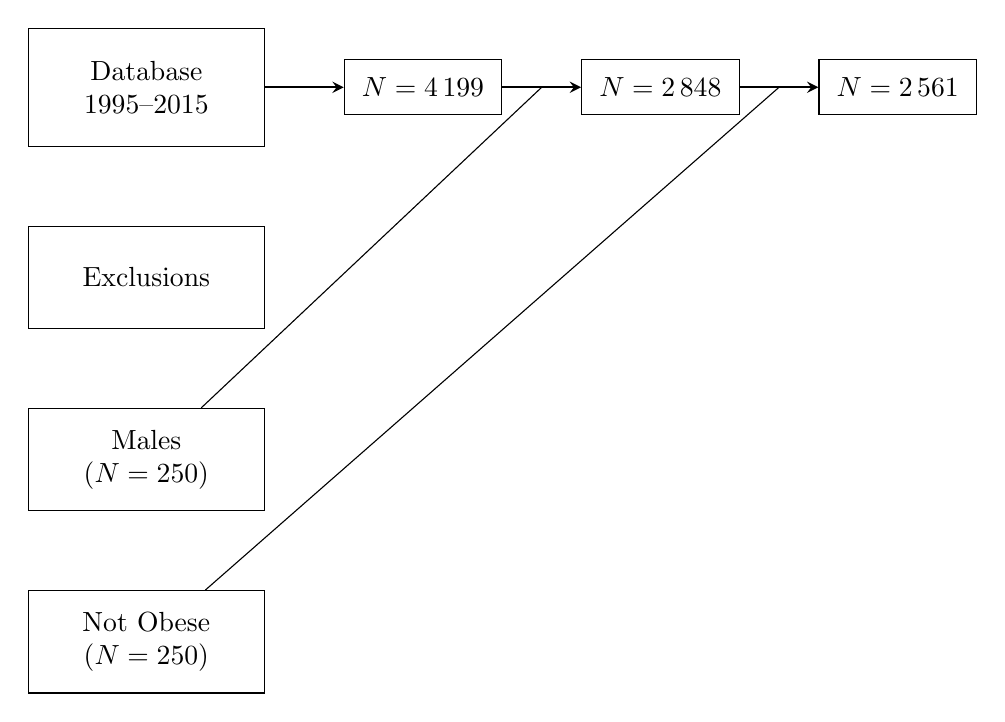
\begin{tikzpicture}%
  [data/.style=
    {draw,minimum height=0.7cm,minimum width=2cm,align=center},
   filter/.style=
    {draw,minimum height=1.3cm,minimum width=3cm,align=center},
   database/.style=
    {draw,minimum height=1.5cm,minimum width=3cm,align=center},
   flow/.style={thick,-stealth},
   apply/.style={}
  ]
  \node[database] (db) {Database\\1995--2015};
  \node[data,right=of db] (d1) {$N=4\,199$};
  \node[data,right=of d1] (d2) {$N=2\,848$};
  \node[data,right=of d2] (d3) {$N=2\,561$};
  \draw[flow] (db) -- (d1);
  \draw[flow] (d1) -- coordinate(d1d2) (d2);
  \draw[flow] (d2) -- coordinate(d2d3) (d3);
  \node[filter,below=of db] (excl) {Exclusions};
  \node[filter, below=of excl] (f1) {Males\\($N=250$)};
  \draw[apply] (d1d2) -- (f1);
  \node[filter, below=of f1] (f2) {Not Obese\\($N=250$)};
  \draw[apply] (d2d3) -- (f2);
\end{tikzpicture}

\end{document}
